% !TEX root =  ../main.tex 

\section{Model for Gleason scores and PSA levels}
The first step in creating a personalized schedule for prostate cancer patients is to come up with a model for Gleason scores, PSA levels and other subject specific characteristics. In PRIAS, PSA levels are measured at the time of induction, every 3 months for the first 2 years in the study and then every 6 months thereafter. Thus PSA levels can be modeled as a longitudinal outcome. As mentioned earlier, patients in PRIAS have a Gleason score of 6 or less at the time of induction in the study, and patients are removed from AS the first time Gleason reclassification takes place. Since our interest also lies in time to Gleason reclassification, we model it as a time to event outcome. i.e. time to Gleason reclassification. \\

While univariate modeling of the two outcomes can be done as mentioned above, our goal is to also utilize the information from PSA levels in deciding the time for scheduling a biopsy. To achieve this, we jointly model time to Gleason reclassification and PSA levels using a joint model for time to event and longitudinal outcomes \cite{rizopoulos2012joint}. 

\subsection{Joint model for time to Gleason reclassification and PSA levels}
Let $T_i^*$ denote the true Gleason reclassification time and $C_i$ denote the censoring time for the $i^{th}$ patient. Let $T_i = \min(T_i^*, C_i)$ denote the observed Gleason reclassification time for the $i^{th}$ patient and $\delta_i = I(T_i^* < C_i)$ is the event indicator. $I(\cdot)$ is the indicator function that takes the value 1 when $T_i^* < C_i$ and 0 otherwise. Let $\boldsymbol{y}_i$ denote the $n_i \times 1$ longitudinal outcome vector for the PSA levels of the $i^{th}$ subject. The population of interest is all the patients enrolled in AS. For a sample of $n$ patients from this population the complete data is denoted by $\mathcal{D}_n = \{T_i, \delta_i, \boldsymbol{y}_i; i = 1,...n\}$.\\

Since both PSA levels and Gleason scores are affected by the state of prostate cancer, they are inherently correlated with each other. In the joint model between time to Gleason reclassification and PSA levels, this correlation between the two outcomes is modeled via a vector of time independent random effects $\boldsymbol{b}_i$. The same random effects are also used to model the correlation between the repeated measurements of the PSA levels. Given the observed PSA history, the censoring process is assumed to be non informative and independent of the time to Gleason reclassification process, as well as of future PSA measurements. With these assumptions, the joint distribution between the two outcomes is given by:

\begin{equation}
p(T_i, \delta_i, \boldsymbol{y}_i | \boldsymbol{b}_i; \theta) = p(T_i, \delta_i | \boldsymbol{b}_i; \theta) p(\boldsymbol{y}_i | \boldsymbol{b}_i; \theta), \text{where}
\end{equation}

\begin{equation}
p(T_i, \delta_i | \boldsymbol{b}_i; \theta) = h_i(T_i|\mathcal{M}_i(T_i); \theta)^{\delta_i} e^{\int_0^{T_i} h_i(s|\mathcal{M}_i(s); \theta) \,ds}, \text{and}
\end{equation}

\begin{equation}
p(\boldsymbol{y}_i | \boldsymbol{b}_i; \theta) = \prod_{j=1}^{n_i} p(y_{ij} | \boldsymbol{b}_i; \theta)
\end{equation}

$\theta = (\theta_t^T, \theta_y^T, \theta_b^T)^T$ denotes the full parameter vector, with $\theta_t$ denoting the parameters for the time to Gleason reclassification outcome, $\theta_y$ the parameters for the PSA levels, and $\theta_b$ the parameters of the random-effects covariance matrix $\boldsymbol{D}$. $\mathcal{M}_i(t) = \{m_i(s), 0\leq s \geq t\}$ denotes the PSA longitudinal history up to time $t$. It is important to note that $m_i(t) = \boldsymbol{x}_i^T(t)\boldsymbol{\beta} + \boldsymbol{z}_i^T(t) \boldsymbol{b}_i$ represent the true value of PSA at time $t$ and not the observed $y_i(t)$. $\boldsymbol{x}_i^T(t)$ and $\boldsymbol{z}_i^T(t)$ are the time dependent design vectors for the fixed effects $\boldsymbol{\beta}$ and random effects $\boldsymbol{b}_i$, respectively.\\ 

The hazard of Gleason reclassification
at any time $t$, given by $h_i(t|\mathcal{M}_i(t);\theta)$ depends on the PSA history $\mathcal{M}_i(t)$ up to the time $t$. Joint models offer flexibility in modeling this dependence. In its simplest form, the hazard may depend on instantaneous value of PSA $m_i(t)$ at time $t$. It is also possible to consider that hazard of Gleason reclassification at time $t$ may depend on PSA velocity $m'_i(t) = \dfrac{d m_i(t)}{dt}$ or $AUC(t) = \int_0^t m_i(s) \,ds$ at the same time. The fact that any functional form of dependence is possible, is evident from the following equation:

\begin{equation}
h_i(t|M_i(t); \theta) = h_0(t) e^{\gamma^Tw_i + f\{M_i(t), \boldsymbol{b}_i, \alpha\}}
\end{equation}

where the function $f(\cdot)$, parametrized by vector $\alpha$ specifies which features of longitudinal outcome process are are included in the linear predictor of the time to event model. For the case at hand, we consider that hazard of Gleason reclassification at any time depends on the PSA value as well as the PSA velocity at the same time. The corresponding hazard function is given by:

\begin{equation}
h_i(t|M_i(t); \theta) = h_0(t) e^{\gamma^Tw_i + \alpha_1 m_i(t) + \alpha_2 m'_i(t)}
\end{equation}

where, $\alpha_1$ and $\alpha_2$ are measures of how strongly hazard of Gleason reclassification depends on PSA value and PSA velocity, respectively. $w_i$ is a vector of time independent covariates and $\gamma$ are the corresponding parameters. $h_0(t)$ is the baseline hazard at time $t$, and is modeled flexibly using a B-splines approach. More specifically:

\begin{equation}
\label{eq : baseline_hazard}
\log h_0(t) = \gamma_{h_0, 0} + \sum_{q=1}^Q  \gamma_{h_0, q} B_q(t, v)
\end{equation}

where $B_q(t, v)$ denotes the $q^{th}$ basis function of a B-spline with knots $v = v_1,...v_Q$ and $\gamma_{h_0}$ the vector of spline coefficients. To avoid choosing the number and position of knots in the spline, a relatively high number of knots (e.g., 15 to 20) are chosen and the corresponding B-spline regression coefficients $\gamma_{h_0}$ are penalized using a differences penalty \cite{eilers1996flexible}.

\subsection{Fitting the joint model to PRIAS dataset}
One of the goals of this work is to compare various scheduling methods for patients of the PRIAS study. We also compare the scheduling methods using a simulation study. For both of these goals, we require parameter estimates of  the joint model between time to Gleason reclassification and PSA levels of PRIAS' patients. For the first goal the parameter estimates are used directly to schedule visits using personalized schedules. For the second goal, we require the parameter estimates of the  joint model to generate data for a simulation study. For these reasons and to also introduce constructs such as dynamic survival probability, we next fit a joint model to the PRIAS data set.\\

The PRIAS data set contains information about 5943 prostate cancer patients who satisfied the conditions for enrollment in AS. For every patient the age at the time of induction in AS was recorded. Other information, namely, PSA levels and Gleason scores were measured at different time points on the basis of a predetermined schedule as mentioned earlier in the report. For the longitudinal analysis of PSA measurements we used $\log_2(PSA + 1)$ measurements instead of the raw data. The log transformation was done because the PSA scores took very large values at the onset of disease progression. This indicated that the underlying distribution for PSA scores was right skewed. Secondly at certain time points patients' PSA scores were measured to be 0, and thus we had to add a constant 1 to all PSA scores before log transformation. We found the same transformation in literature as well \cite{mcgreevy2006impact,sene2016individualized}. For the variable Age in the Cox model, we wanted to  consider both the linear and quadratic effect. However doing so led many numerical instabilities while performing the joint model analysis. To avoid these pitfalls we had to center the Age variable around age 70 years. The longitudinal and survival submodels of the joint model we fitted is given by:

\begin{align*}
\log_2\{PSA + 1\}(t) &= m_i(t) + \varepsilon_i(t), \\
m_i(t) &= (\beta_0 + b_{i0}) + \beta_1 (Age-70) + \beta_2 (Age-70)^2\\ 
&+ \sum_{k=1}^4 \beta_{k+2} B_k(t,\mathcal{K}) + b_{i1} B_7(t, 0.5) + b_{i2} B_8(t, 0.5) \\
\varepsilon_i(t) & \sim N(0, \sigma^2),\\
\boldsymbol{b}_i & \sim N(0, \boldsymbol{D})
\end{align*}

The evolution of PSA levels over time is modeled flexibly using B-splines. For the fixed effects part the spline consists of 3 internal knots. The internal knots are at $\mathcal{K} =\{0.5, 1.2, 2.5\}$ years, and boundary knots are at 0 and 7 years. For the random effects part there is only 1 internal knot at 0.5 years and the boundary knots are at 0 and 7 years. The choice of knots was based on exploratory analysis as well as on the basis of model selection criteria AIC and BIC. For the survival submodel the hazard function we fitted is given by:

\begin{equation}
h_i(t) = h_0(t) e^{\gamma_1 (Age-70)  + \gamma_2 (Age-70)^2  \alpha_1 m_i(t) + \alpha_2 m'_i(t)}
\end{equation}

The baseline hazard $h_0(t)$ is modeled as in equation \ref{eq : baseline_hazard}. To fit the joint model we use the R package JMbayes \cite{rizopoulosJMbayes}, which uses a Bayesian approach for parameter estimation. The parameter estimates for the survival submodel were estimated using Bayesian ridge methodology.

\subsubsection{Parameter Estimates}
The parameter estimates for the joint model we fitted to the PRIAS data set are shown in Table \ref{tab : PSA_long} and Table \ref{tab : PSA_survival}. Since the longitudinal evolution of $\log_2(PSA + 1)$ is modeled with non-linear terms, the interpretation of the coefficients corresponding to time is not straightforward. In lieu of the interpretation we present the fitted evolution of PSA over a period of 10 years for a patient who is 70 years old in Figure \ref{fig : fitted_trend_psa}. It can be seen that the after the first 6 months the PSA levels steadily increase over the follow up period. Since the model for PSA has only additive terms, this evolution remains same for all patients. The effect of Age only affects the baseline PSA score. However it is so small that it can be ignored for all practical purposes.\\

\begin{figure}[!htb]
	\centering
    \captionsetup{justification=centering}
	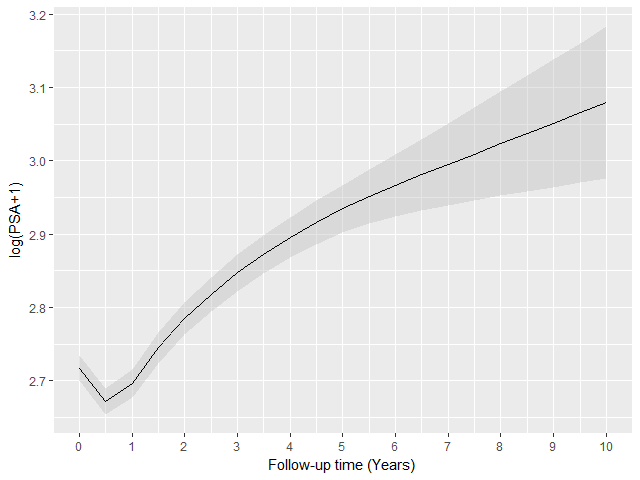
\includegraphics[width=0.8\textwidth]{fitted_trend_psa.png}
	\caption{Fitted evolution of $\log_2(PSA+1)$ over a period of 10 years, for a patient who was inducted in AS at the Age of 70 years.}
	\label{fig : fitted_trend_psa}
\end{figure}

\begin{table}[!htb]
\centering
\caption{Longitudinal submodel estimates for joint model.}
\label{tab : PSA_long}
\captionsetup{justification=centering}
\begin{tabular}{@{}lrrrrr@{}}
\toprule
                                     & Mean   & Std. Dev           & 2.5\%               & 97.5\%              & P              \\ \midrule
Intercept                            & 2.717  & 0.008              & 2.701               & 2.733               & \textless0.000 \\
(Age - 70)                           & 0.003  & 0.001              & 0.001               & 0.005               & 0.002          \\
(Age - 70) $\times$ (Age - 70)       & -0.001 & 1 $\times 10^{-4}$ & -7 $\times 10^{-4}$ & -4 $\times 10^{-4}$ & \textless0.000 \\
Spline: visitTimeYears{[}0, 0.5{]}   & 0.026  & 0.008              & 0.012               & 0.042               & \textless0.000 \\
Spline: visitTimeYears{[}0.5, 1.2{]} & 0.208  & 0.013              & 0.184               & 0.233               & \textless0.000 \\
Spline: visitTimeYears{[}1.2, 2.5{]} & 0.175  & 0.019              & 0.137               & 0.210               & \textless0.000 \\
Spline: visitTimeYears{[}2.5, 7{]}   & 0.309  & 0.028              & 0.256               & 0.366               & \textless0.000 \\
$\sigma$                               & 0.273  & 0.001              & 0.271               & 0.275               & \textless0.000 \\ \bottomrule
\end{tabular}
\end{table}

For the survival submodel, the parameter estimates in Table \ref{tab : PSA_survival} show that both the $\log_2(PSA + 1)$ value and $\log_2(PSA + 1)$ velocity are associated with time to Gleason reclassification. The effect is quite strong and if at any given time point the PSA becomes approximately 4 times of its value then the hazard of Gleason reclassification  becomes 1.5 times of the original. This is valid under the condition that the $\log_2(PSA + 1)$ velocity remains the same. The effect of $\log_2(PSA + 1)$ velocity is far stronger, but it is not interpretable easily. Lastly, for the effect of Age on hazard we can say that it can be safely ignored for all practical purposes.

\begin{table}[!htb]
\centering
\caption{Survival submodel estimates for joint model.}
\captionsetup{justification=centering}
\label{tab : PSA_survival}
\begin{tabular}{@{}lrrrrr@{}}
\toprule
Variable                      & Mean   & Std. Dev & 2.5\%  & 97.5\%                 & P              \\ \midrule
Age - 70                      & 0.036  & 0.007    & 0.023  & 0.050                  & \textless0.000 \\
(Age - 70) $\times$ (Age - 70) & -0.002 & 0.001    & -0.004 & 2 $\times 10^{-4}$ & 0.016          \\
$\log_2(PSA + 1)$                  & 0.184  & 0.093    & 0.016 & 0.369                  & 0.032          \\
Slope: $\log_2(PSA + 1)$           & 1.937  & 0.278    & 1.420  & 2.525                  & \textless0.000 \\ \bottomrule
\end{tabular}
\end{table}

\subsubsection{Dynamic survival probability}
\label{subsubsec: dyn_surv_prob}
Since patients' PSA levels and Gleason scores are periodically measured, the entire PSA and repeat biopsy history can be used to periodically update the predictions about about time to Gleason reclassification. More specifically, let us assume that a new patient numbered $j$, not present in the original sample of patients $\mathcal{D}_n$, did not have a Gleason reclassification at their last biopsy, performed at time $t$. Further, let us assume that the PSA measurements are available for the patient $j$ up to a time point $s > t$. Then combining these two pieces of information, the distribution for time to Gleason reclassification for this patient is given by:

\begin{equation}
p(T^*_j | T^*_j > t, \mathcal{Y}_j(s), \mathcal{D}_n; \theta^*)
\end{equation}

where $\mathcal{Y}_j(s) = \{y_j(r); 0 \leq r \leq s\}$ denotes the history of PSA measurements done up to time $s$. The personalized schedules we propose in this work depend on this dynamic distribution for time to Gleason reclassification. As more PSA measurements are taken and repeat biopsies are performed, this distribution is accordingly updated. The survival probabilities based on this distribution are called dynamic survival probabilities \cite{rizopoulos2011dynamic}. The dynamic survival probability at any time point $u > s$ is given by:

\begin{equation}
\pi_j(u|t) = Pr(T^*_j \geq u| T^*_j >t, \mathcal{Y}_j(s), D_n; \theta)
\end{equation}

\begin{figure}[!htb]
	\centering
    \captionsetup{justification=centering}
	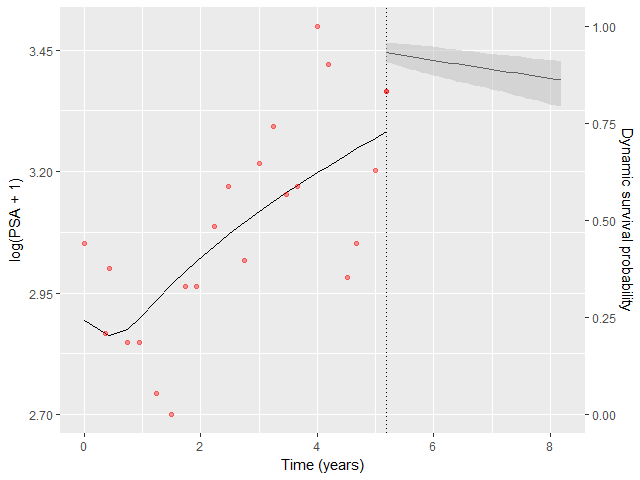
\includegraphics[width=0.8\textwidth]{dyn_surv_prob_2362.png}
	\caption{Dynamic survival probability for patient with ID 2362 in the PRIAS data set.}
	\label{fig : dyn_surv_prob_2362}
\end{figure}

As an example we present the dynamic survival probability of patient 2362 from the PRIAS data set. Patient 2362 had his last repeat biopsy at 3.78 years at which the Gleason reclassification did not happen. The patient was later censored at 5.12 years. Using all this information up to 5.12 years, the dynamic survival probability at any time point $u > 3.78$ for this patient is given by the formula $Pr(T^*_{2362} \geq u| T^*_{2362} > 3.78, \mathcal{Y}_{2362}(5.12), D_n; \theta)$. Figure \ref{fig : dyn_surv_prob_2362} shows the dynamic survival probability for patient 2362 at time points between 5.12 and 8.12 years.